                                                           
% \begin{abstract}
% In this paper, we propose a novel neural approach for paraphrase generation. Conventional paraphrase generation methods either leverage hand-written rules and thesauri-based alignments, or use statistical machine learning principles. To the best of our knowledge, this work is the first to explore deep learning models for paraphrase generation. Our primary contribution is a stacked residual LSTM network, where we add residual connections between LSTM layers. This allows for efficient training of deep LSTMs. We experiment with our model and other state-of-the-art deep learning models on three different datasets: \texttt{PPDB}, \texttt{WikiAnswers} and \texttt{MSCOCO}. Evaluation results demonstrate that our model outperforms sequence to sequence, attention-based and bi-directional LSTM models on \texttt{BLEU}, \texttt{METEOR}, \texttt{TER} and an \emph{embedding}-based sentence similarity metric.
% \end{abstract}
 
\section{Introduction}
 
 
Paraphrasing, the act of using textual alternatives to express the same meaning as the source content, is an important subtask in various Natural Language Processing (NLP) applications such as question answering, information extraction, information retrieval, summarization and natural language generation. Research on paraphrasing methods typically aims at solving three related problems: (1) recognition (i.e.\ to identify if two textual units are paraphrases of each other), (2) extraction (i.e.\ to extract paraphrase instances from a thesaurus or a corpus), and (3) generation (i.e.\ to generate a reference paraphrase given a source textual unit) \cite{Madnani2010}. In this paper, we focus on the paraphrase generation problem.
 
Paraphrase generation has been used to gain performance improvements in several NLP applications, for example, by generating query variants or pattern alternatives for information retrieval, information extraction or question answering systems, by creating reference paraphrases for automatic evaluation of machine translation and document summarization systems, and by generating concise or simplified information for sentence compression or sentence simplification systems \cite{Madnani2010}.
 
Traditional paraphrase generation methods exploit hand-crafted rules \cite{McKeown1983} or automatically learned complex paraphrase patterns \cite{Zhao2009}, use thesaurus-based \cite{Hassan2007} or semantic analysis driven natural language generation approaches \cite{Kozlowski2003}, or leverage statistical machine learning theory \cite{quirk2004,Wubben2010}. In this paper, we propose to use deep learning principles to address the paraphrase generation problem.
Recently, techniques like sequence to sequence learning \cite{SutskeverVL14} have been applied to various NLP tasks with promising results, for example, in the areas of machine translation \cite{cho14,Bahdanau15}, speech recognition \cite{li2015constructing}, language modeling \cite{vinyals2015grammar}, and dialogue systems \cite{serban2016multiresolution}. Although paraphrase generation can be formulated as a sequence to sequence learning task, not much work has been done in this area with regard to applications of state-of-the-art deep neural networks. There are several works on paraphrase recognition \cite{SocherEtAl2011,yin-schutze2015,kiros2015skip}, but those employ classification techniques and do not attempt to generate paraphrases. Another recent related work uses attention-based Long Short-Term Memory (LSTM) networks for textual entailment generation \cite{KolesnykRR16}; however, paraphrase generation is a type of bidirectional textual entailment generation and no prior work has proposed a deep learning-based formulation of this task.
In the light of the lack of such prior work, we explore various types of sequence to sequence models for paraphrase generation. We test these models on three different datasets and evaluate these models using various metrics. Along with the application of various existing sequence to sequence models for the paraphrase generation task, in this paper we also propose a new model that allows for training multiple stacked LSTM networks by introducing a residual connection between the layers. This is inspired by the recent success of such connections in a deep Convolutional Neural Network (CNN) for the image recognition task \cite{he2015deep}. Our experiments demonstrate that the proposed model can outperform various other techniques we have explored.
Most of the deep learning models in NLP use Recurrent Neural Networks (RNNs). RNNs differ from normal perceptrons as they allow gradient propagation in time to model sequential data with variable-length input and output \cite{SutskeverMH11}. In practice, RNNs often suffer from the vanishing/exploding gradient problems while learning long-range dependencies \cite{Bengio94}. LSTM \cite{Hochreiter:1997} and GRU \cite{cho14} are known to be successful remedies to these problems.
It has been observed that increasing the depth of a deep neural network can improve the performance of the model \cite{Simonyan2014VeryDC,he2015deep} as deeper networks learn better representations of features \cite{farabet2013learning}. In the vision related tasks where CNNs are more widely used, adding many layers of neurons is a common practice. For tasks like speech recognition \cite{li2015constructing} and also in machine translation, it is useful to stack layers of LSTM or any other variants of RNN.\ So far this has been limited to only a few layers due to difficulty in training deep RNN networks. We propose to add residual connections between multiple stacked LSTM networks and show that this allows us to stack more layers of LSTM successfully.
 
The rest of the paper is organized as follows: Section 2 presents a brief overview of the sequence to sequence models followed by a description of our proposed residual deep LSTM model, Section 3 describes the datasets used in this work, Section 4 explains the experimental setup, Section 5 presents the evaluation results and analyses, Section 6 discusses the related work, and finally, in Section 7 we conclude and discuss future work.
 
 
\section{Model Description}
\subsection{Encoder-Decoder Model}
A neural approach to sequence to sequence modeling proposed by Sutskever et al.~\cite{SutskeverVL14} is a two-component model, where a source sequence is first encoded into some low dimensional representation (Figure~\ref{fig:enc_dec}) that is later used to reproduce the sequence back to a high dimensional target sequence (i.e.\ decoding). In machine translation, an encoder operates on text written in the source language and encodes the meaning of the sentence to be translated before the decoder can take that vector (which represents the meaning) and generate a sentence in the target language. These encoder-decoder blocks can be either a vanilla RNN or its variants. While producing the target sequence, the generation of each new word depends on the model and the last word generated. For the first word, this is done by appending a special `\texttt{EOS}' (end-of-sentence) token to the source.
The training objective is to maximize the log probability of the target sequence given the source sequence. Therefore, the best possible decoded target is the one that has the maximum score over the length of the sequence. To find this, a small set of hypotheses (candidate set) called \emph{beam size} is used and the total score for all these hypotheses are computed. In the original work by Sutskever et al.~\cite{SutskeverVL14}, they observe that even beam size of $1$ gives a very good result but a higher beam size always does better. This is because for some of the hypotheses the first word may not have the highest score.

\begin{figure}
    \centering
    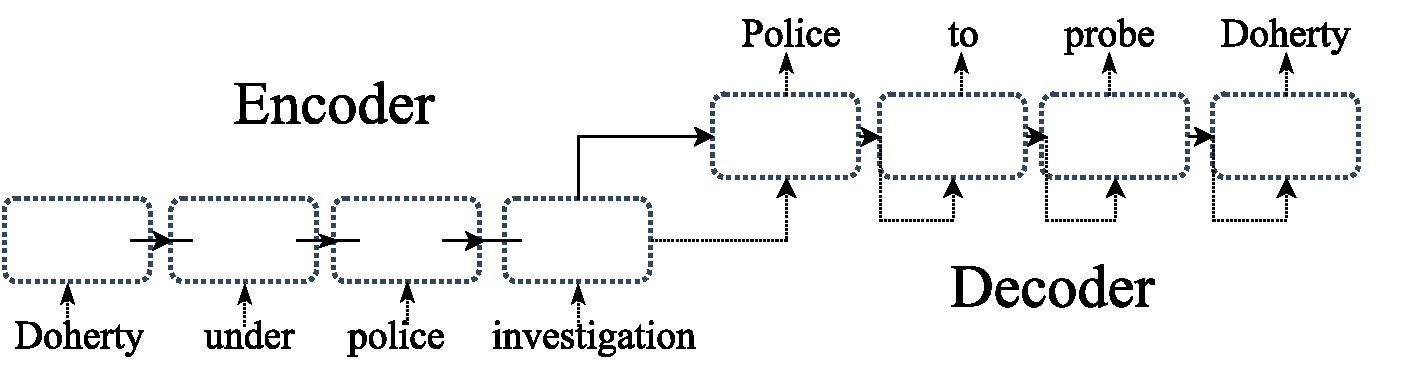
\includegraphics[scale=0.5]{figures/paraphrase/seq2seq.pdf}
    \caption[Sequence to Sequence Learning]{Encoder-Decoder framework for sequence to sequence learning}
    \label{fig:enc_dec}
\end{figure}
 
\subsection{Deep LSTM}
LSTM (Figure~\ref{fig:lstmcell}) is a RNN which adds an internal memory cell $c_t \! \in \! \mathbb{R}^n$ at every time step. An LSTM unit takes three inputs $x_t,h_{t-1},c_{t-1}$ at every time step and produces the hidden state, $h_t$ and the internal memory state, $c_t$ at time step $t$. The memory cell is controlled via three learned gates: input $i$, forget $f$, and output $o$. These memory cells use the addition of gradient with respect to time and thus minimize the gradient explosion. In most NLP tasks, LSTM outperforms vanilla RNN \cite{sundermeyer2012lstm}. Therefore, for our model we only explore LSTM as a basic unit in the encoder and decoder. Here, we describe the basic computations in an LSTM unit, which will provide the grounding to understand the residual connections between stacked LSTM layers later.
In the equations below, $W_{x\_}, W_{h\_}$ are the learned parameters for $x$ and $h$ respectively. $\sigma(.)$ and $\tanh(.)$ denote element-wise sigmoid and hyperbolic tangent functions. $\astrosun$ is the element-wise multiplication operator and $b$ denotes the added bias.

\begin{enumerate}
  \item Gates \\
        \(\displaystyle   i_{t} = \sigma(W_{xi}x_{t} + W_{hi}h_{t-1} + b_{i}) \) \\
        \(\displaystyle   f_{t} = \sigma(W_{xf}x_{t} + W_{hf}h_{t-1} + b_{f}) \) \\
        \(\displaystyle   o_{t} = \sigma(W_{xo}x_{t} + W_{ho}h_{t-1} + b_{o}) \) 
  \item Input transform \\
        \(\displaystyle    c\_in_{t} = \textrm{tanh}(W_{xc}x_{t} + W_{hc}h_{t-1} + b_{c\_in})  \) 
  \item State Update \\
        \(\displaystyle    c_{t} = f_{t} \ \astrosun \ c_{t-1} + i_{t} \ \astrosun c\_in_{t} \) \\
        \(\displaystyle    h_{t} = o_{t} \ \astrosun \ \textrm{tanh}(c_{t}) \) 
 
\end{enumerate}

\begin{figure}
    \centering
    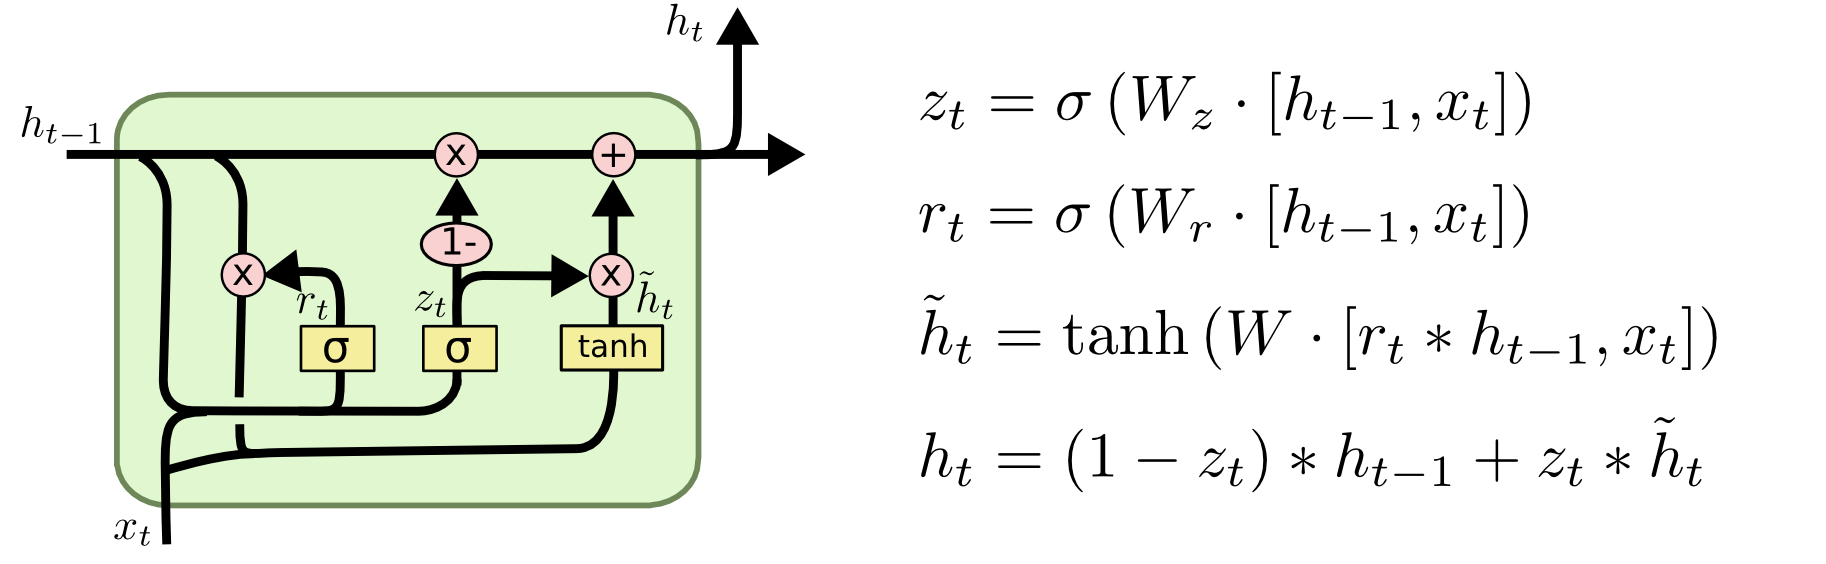
\includegraphics[scale=0.7]{figures/paraphrase/lstm_cell.png}
    \caption{LSTM Cell. Fig reproduced with permission from Chris Olah}
    \label{fig:lstmcell}
\end{figure}
 
 
% \subsection{ Deep LSTM }
Graves~\cite{graves2013generating} explored the advantages of deep LSTMs for handwriting recognition and text generation. There are multiple ways of combining one layer of LSTM with another. For example, Pascanu et al.~\cite{pascanu2013construct} explored multiple ways of combining them and discussed various difficulties in training deep LSTMs. In this work, we employ vertical stacking where only the output of the previous layer of LSTM is fed to the input, as compared to
the stacking technique used by Sutskever et al.~\cite{SutskeverVL14}, where hidden states of all LSTM layers are fully connected. In our model, all but the first layer input at time step $t$ is passed from the hidden state of the previous layer $h_{t}^{l}$, where $l$ denotes the layer. This is similar to stacked RNN proposed by Bengio et al.~\cite{Bengio94} but with LSTM units. Thus, for a layer $l$ the activation is described by:
$$
\bm{h}_{t}^{(l)} = f_{h}^{l}(\bm{h}_{t}^{(l-1)}, \bm{h}_{t-1}^{(l)})
$$
where hidden states $\bm{h}$ are recursively computed and $\bm{h}_{t}^{(l)} $ at $t=0$ and $l=0$ is given by the LSTM equation of $h_{t}$.
 
\subsection{Stacked Residual LSTM}
We take inspiration from a very successful deep learning network \emph{ResNet} \cite{he2015deep} with regard to adding residue for the purpose of learning. With  theoretical and empirical reasoning, He et al.~\cite{he2015deep} have shown that the explicit addition of the residue $x$ to the function being learned allows
for deeper network training without overfitting the data.
 
When stacking multiple layers of neurons, often the network suffers through a \emph{degradation} problem \cite{he2015deep}. The degradation problem arises due to the low convergence rate of training error and is different from the vanishing gradient problem. Residual connections can help overcome this issue. We experimented with four-layers of stacked LSTM for each of the model. Residue connections is added at layer two as the pointwise addition (see Figure~\ref{fig:res}), and thus it requires the input to be in the same dimension as the output of $h_t$. Principally because of this reason, we use a simple last hidden unit stacking of LSTM instead of a more intricate way as shown by Sutskever et al.~\cite{SutskeverVL14}. This allowed us to clip the $h_t$ to match the dimension of $x_{t-2}$ where they were not the same. Similar results could be achieved by padding $x$ to match the dimension instead. The function $\bm{\hat{h}}$ that is being learned for the layer with residue connection is therefore:
$$
\bm{\hat{h}}_{t}^{(l)} = f_{h}^{l}(\bm{h}_{t}^{(l-1)}, \bm{h}_{t-1}^{(l)}) + x_{l-n}
$$
where $\hat{h}$ for layer $l$ is updated with residual value $x_{l-n} $ and $x_{i}$ represents the input to layer $i+1$. Residual connection is added after every $n$ layers. However, for stacked LSTM $n>3$ is very expensive in terms of computation. In this paper we experimented with $n=2$. Note that when $n=1$, the resulting function learned is a standard LSTM with bias that depends on the input $x$. That is why, it is not necessary to add the residue connection after every stacked layer of LSTM.\ Addition of residual connection does not add any learnable parameters. Therefore, this does not increase the complexity of model unlike bi-directional models which doubles the number of LSTM units.
\begin{figure}
    \centering
    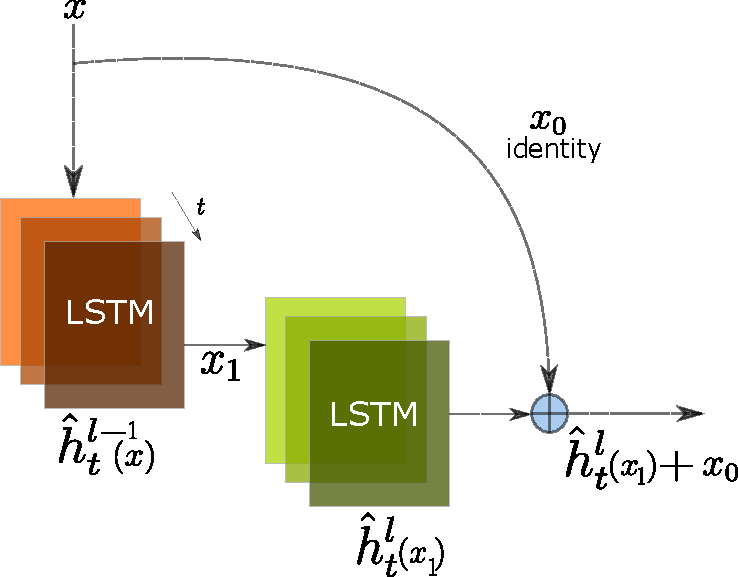
\includegraphics[scale=0.8]{figures/paraphrase/reslstm.pdf}
    \caption[Residual LSTM]{A unit of stacked residual LSTM}
    \label{fig:res}
\end{figure}
 
\section{Datasets}
We present the performance of our model on three datasets, which are significantly different in their characteristics.
\textbf{PPDB} \cite{pavlick2015} is a well known dataset used for various NLP tasks. It comes in different sizes and the precision of the paraphrases degrades with the size of the dataset. We use the size $L$ dataset from \texttt{PPDB} 2.0, which comes with over $18M$ paraphrases including lexical, phrasal and syntactic types. We have omitted the syntactic paraphrases and the instances which contain numbers, as they increase the vocabulary size significantly without giving any advantage of a larger dataset. This dataset contains relatively short paraphrases ($86\%$ of the data is less than four words), which makes it suitable for synonym generation and phrase substitution to address lexical and phrasal paraphrasing \cite{Madnani2010}. For some phrases, \texttt{PPDB} has one-to-many paraphrases. All such phrases were collected to make a set of paraphrases and sampling without replacement was used to obtain the source and reference phrases.
 
\textbf{WikiAnswers} \cite{fader2013paraphrase} is a large question paraphrase corpus created by crawling the WikiAnswers website, where users can post questions and answers about any topic. The paraphrases are different questions, which were tagged by the users as similar questions. The dataset contains approximately 18M word-aligned question pairs. There is some loss of specialization between the given source question (a paraphrase to be tagged as similar to the reference question) and the reference question. For example, ``prepare a \emph{three month} cash budget'' is tagged to ``how to prepare a cash budget''. This happens because it is more likely that a general question has been answered as they are more popular and specific ones are redirected to the general ones due to comparative lack of interest in a very specific question. It should be noted that this dataset has been lemmatized and some processing has been done in order to sanitize the large corpus. We refer the reader to the original paper for more details.
\textbf{MSCOCO} \cite{lin2014microsoft} dataset contains human annotated captions of over $120K$ images. Each image contains five captions from five different annotators. While there is no guarantee that the human annotations are paraphrases, but because of the nature of the image (which tends to focus on only a few objects and in most cases one prominent object or action) most annotators describe the obvious thing in the image. In fact, this is the main reason why neural networks for generating captions obtain very good \texttt{BLEU} scores \cite{VinyalsTBE14}, which allows us to use this dataset for the paraphrase generation task.
 
 
%In this regard, our model works like a blind captioner to generate captions only using other captions and not the image.
 
\section{Experimental Settings}
\subsection{Data Selection}
For \texttt{PPDB} we remove the phrases that contain numbers, which includes all syntactic phrases. This step gives us a total of $5.3M$ paraphrases from which we randomly select $90\%$ instances for training and $20K$ pairs from the rest $10\%$ data are selected similarly for testing. Although \texttt{WikiAnswers} comes with $29,139,992$ instances, we randomly select $4,826,492$ for training to keep the training size similar to \texttt{PPDB} (see Table 1). $20K$ instances are randomly selected from the remaining data for testing. Note that, for the \texttt{WikiAnswers} dataset, we had to clip the vocabulary size\footnote{\texttt{WikiAnswers} dataset had many spelling errors yielding a very large vocabulary size (approximately $250K$). Hence, we selected the most frequent $50K$ words in the vocabulary to reduce the computational complexity.} to $50K$ and use the special \emph{UNK} symbol for the words outside the vocabulary. \texttt{MSCOCO} dataset has five captions for every image. This dataset comes with separate subsets for training and validation: \emph{Train 2014} contains over $82K$ images and \emph{Val 2014} contains over $40K$ images. From each set of five captions, we randomly select two pairs to use as training instances. The remaining caption is disregarded. Because of the free form nature of the caption generation task \cite{VinyalsTBE14}, some captions were very long. We clipped those captions to the size of $15$ words in order to make the training feasible.

\begin{table}
    \rowcolors{1}{White}{Gray}
      \centering
    \begin{tabular}{lllr}
    \midrule
    \multicolumn{1}{c}{\textbf{Dataset}} & \multicolumn{1}{c}{\textbf{Training}} & \multicolumn{1}{c}{\textbf{Test}} & \multicolumn{1}{c}{\textbf{Vocabulary Size}}\\
    \midrule
    \texttt{PPDB}                        & 4,826,492                    & 20,000         & 38,279          \\
    \texttt{WikiAnswers}                 & 4,826,492                    & 20,000         & 50,000          \\
    \texttt{MSCOCO}                      & 331,163                      & 20,000         & 30,332         \\
    \midrule
    \end{tabular}
     \caption{Dataset details}
\end{table}

\begin{table}
      \centering
        \rowcolors{1}{White}{Gray}
        \begin{tabular}{ll}
        \midrule
        \textbf{Models}                                      & \textbf{Reference}  \\
        \midrule
        Sequence to Sequence                                 & \cite{SutskeverVL14} \\
        With Attention                                       & \cite{Bahdanau15} \\
        Bi-directional LSTM                                  & \cite{graves2013hybrid} \\
        Residual LSTM                                        & Our proposed model                                   \\             
        \midrule
        \end{tabular}
        \caption{Models}
\end{table}


\begin{figure}
    \centering
    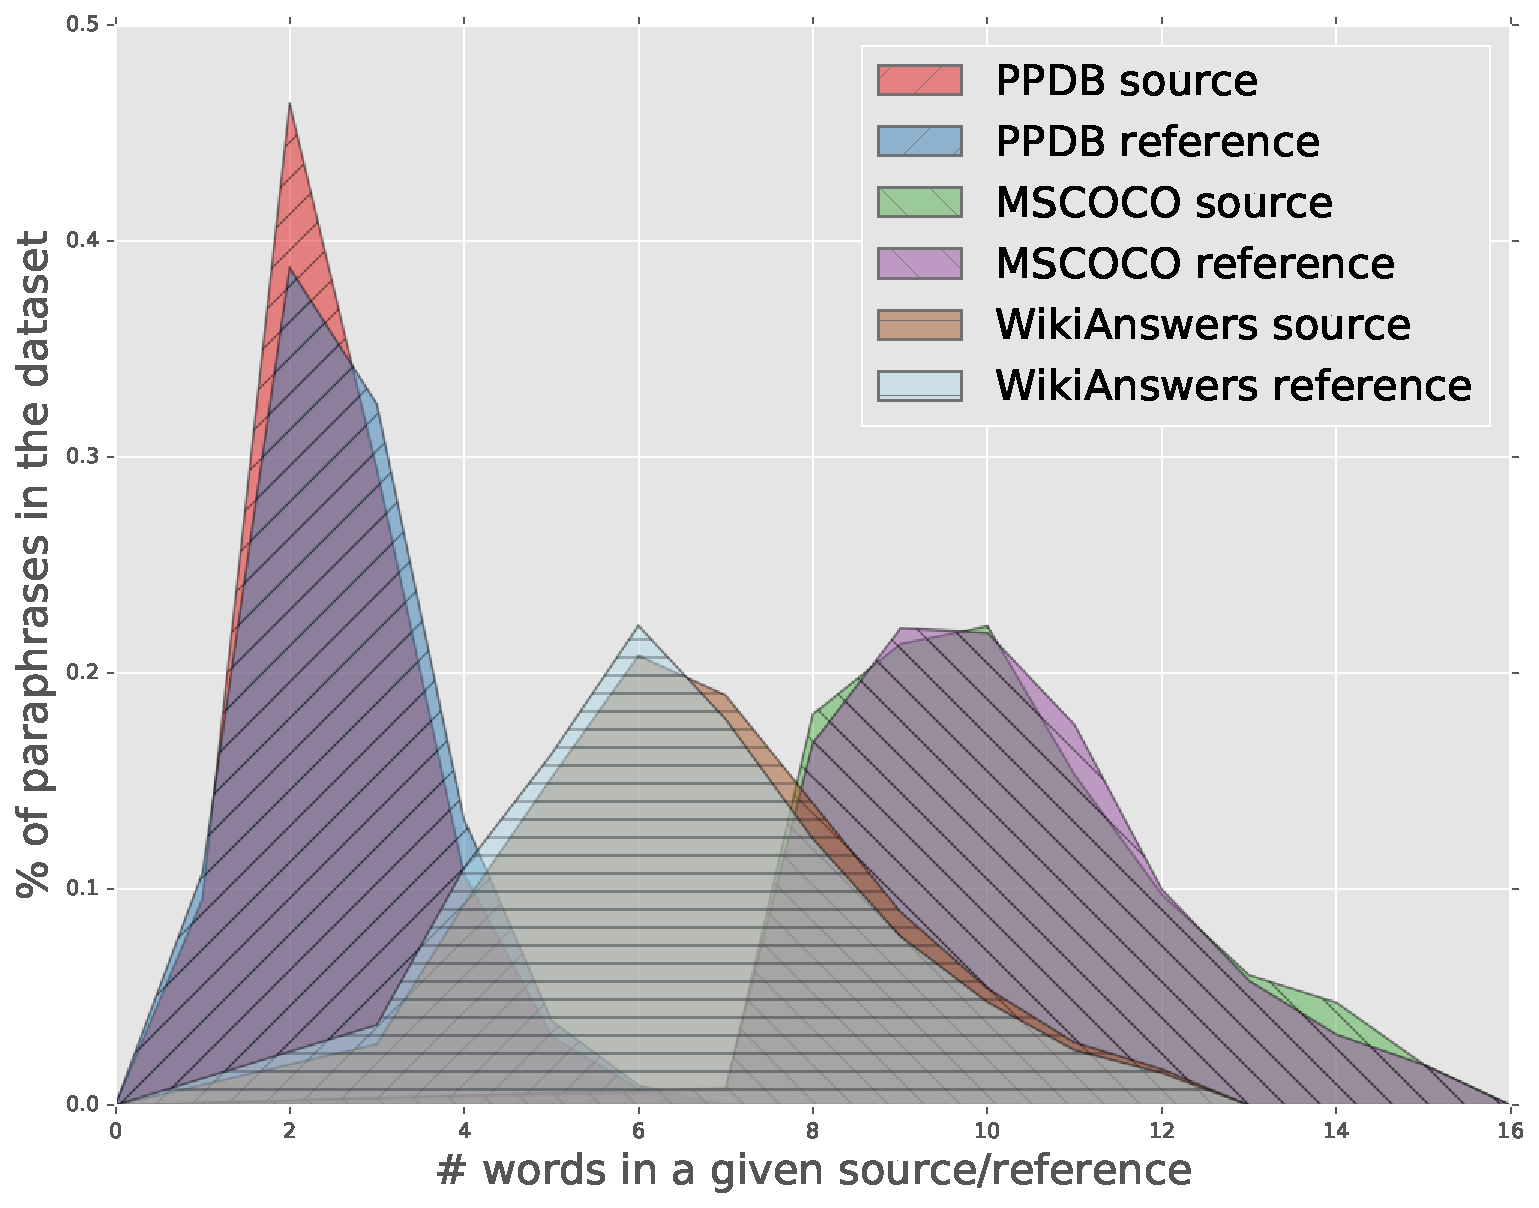
\includegraphics[scale=0.50]{figures/paraphrase/wordlength.pdf}
    \caption[Distribution of word length]{Distribution of word length across datasets}
    \label{fig:res1}
\end{figure}

 
\subsection{Models}
In this work, we experimented with four different models (see Table 2). For each model, we experimented with two- and four-layers of stacked LSTMs. This was motivated from the state-of-the-art speech recognition systems that also use three to four layers of stacked LSTMs \cite{li2015constructing}. In encoder-decoder models, the size of the beam search used during inference is very important. Larger beam size always give higher accuracy but comes at a computational cost. We experimented with beam sizes of $5$ and $10$ to compare the models, as these are the most common beam sizes used in the literature \cite{SutskeverVL14}. The bi-directional model used half of the number of layers shown for other models. This was done to ensure similar parameter sizes across the models.
 
\subsection{Training}
We used a one-hot vector approach to represent the words in all models. Models were trained with a stochastic gradient descent (SGD) algorithm. The learning rate began at $1.0$, and was halved after every third training epoch. Each network was trained for ten epochs. A standard dropout \cite{srivastava2014dropout} of 50\% was applied after every LSTM layer. The number of LSTM units in each layer was fixed to $512$ across all models. In order to allow exploration of a wide variety of models, training was restricted to a limited number of epochs, and no hyper-parameter search was performed. Training time ranged from $36$ hours for \texttt{WikiAnswers} and \texttt{PPDB} to $14$ hours for \texttt{MSCOCO} on a \emph{Titan X} with \emph{CuDNN 5} using Theano version $0.9.0dev1$ \cite{2016arXiv160502688short}.
 
A beam search algorithm was used to generate optimal paraphrases by exploiting the trained models in the testing phase \cite{SutskeverVL14}. We used perplexity as the loss function during training. Perplexity measures the uncertainty of the language model, corresponding to how many bits on average would be needed to encode each word given the language model. A lower \texttt{PPLX} indicates a better score. While \texttt{WikiAnswers} and \texttt{MSCOCO} had a very good correlation of training and validation perplexity, \texttt{PPDB} easily overfitted and did not yield good validation perplexity (see Figure~\ref{fig:perplex}).
\begin{figure}
    \centering
    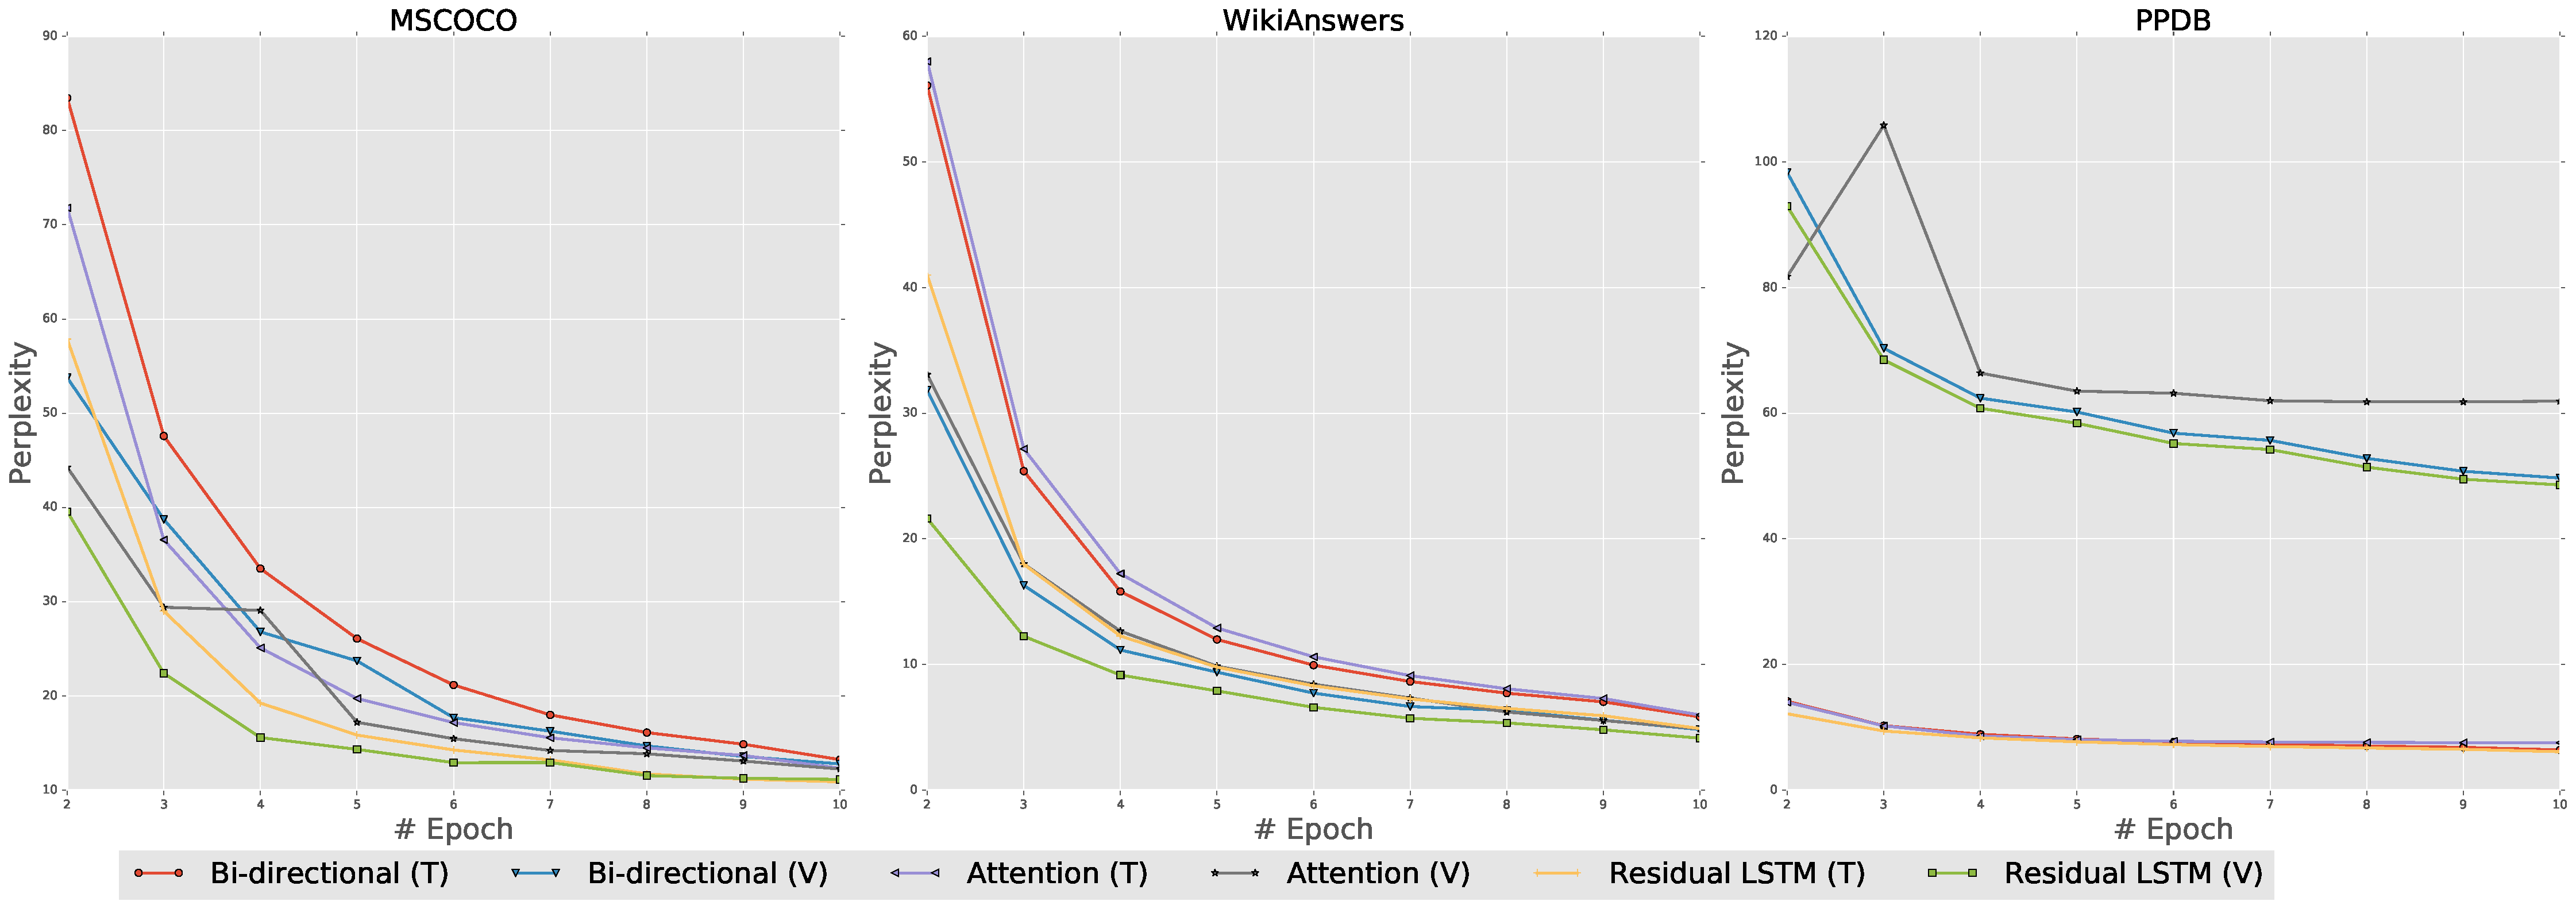
\includegraphics[scale=0.25]{figures/paraphrase/plots.pdf}
    \caption[Model Evaluation]{Perplexity ($\downarrow$) during training and validation for various models [shared legend]}
    \label{fig:perplex}
\end{figure}
\section{Evaluation}
\subsection{Metrics}
To quantitatively evaluate the performance of our paraphrase generation models, we use the well-known automatic evaluation metrics\footnote{We used the software available at \url{https://github.com/jhclark/multeval}} for comparing parallel corpora:
\texttt{BLEU} \cite{papineni2002}, \texttt{METEOR}  \cite{Lavie2007}, and Translation Error Rate (\texttt{TER}) \cite{snover2006study}. Even though these metrics were designed for machine translation, previous works have shown that they can perform well for the paraphrase recognition task \cite{Madnani2012} and correlate well with human judgments in evaluating generated paraphrases \cite{Wubben2010}.
 
Although there exists a few automatic evaluation metrics that are specifically designed for paraphrase generation, such as \texttt{PEM} (Paraphrase Evaluation Metric) \cite{LiuDN10} and \texttt{PINC} (Paraphrase In N-gram Changes) \cite{ChenD11}, they have certain limitations. \texttt{PEM} relies on large in-domain bilingual parallel corpora along with sample human ratings for training the metric and it can only model paraphrasing up to the phrase-level granularity. \texttt{PINC} attempts to solve these limitations by proposing a method that is essentially the inverse of \texttt{BLEU}, as it calculates the n-gram difference between the source and the target sentences. Although \texttt{PINC} correlates well with human judgments in lexical dissimilarity assessment, \texttt{BLEU} have been shown to correlate better for semantic equivalence agreements at the sentence-level when a sufficiently large number of reference sentences are available for each source sentence \cite{ChenD11}.
 
\texttt{BLEU} considers exact matching between reference paraphrases and system generated paraphrases by considering n-gram overlaps while \texttt{METEOR} improves upon this measure via stemming and synonymy using WordNet. \texttt{TER} measures the number of edits required to change a system output into one of the references. As suggested in \cite{Clark:2011}, we used a stratified approximate randomization (AR) test. AR calculates the probability of a metric score providing the same reference sentence by chance. We report our {\it p}-values at \texttt{95\%} Confidence Intervals (CI).
The major limitation of these evaluation metrics is that they do not consider the meaning of the paraphrases, and hence, are not able to capture paraphrases of entities. For example, these metrics will not reward the paraphrasing of \emph{Coke} to \emph{Pepsi}. However, in Word2Vec embeddings they will be considered as similar entities. Therefore, we also evaluate our models on a sentence similarity metric\footnote{We used the software available at \url{https://github.com/julianser/hed-dlg-truncated/}} proposed by Rus et al.~\cite{rus2012comparison}. This metric uses word embeddings to compare the phrases. In our experiments, we used Word2Vec embeddings pre-trained on the Google News Corpus \cite{mikolov2014word2vec}. This is referred as \emph{`Emb Greedy'} in our results table.
\subsection{Results}
\begin{table}[htbp]
\centering
\footnotesize
\rowcolors{1}{White}{Gray}
\hspace*{-6em}
\begin{tabular}{rlll}
\midrule
\multicolumn{1}{l}{}           & \multicolumn{1}{l}{{\texttt{PPDB}}}                                  & \multicolumn{1}{l}{{\texttt{WikiAnswers}}}                                                       & \multicolumn{1}{l}{{\texttt{MSCOCO}}}                              \\ \hline
\multicolumn{1}{r|}{\textbf{Src}}    & \multicolumn{1}{l||}{south eastern}    & \multicolumn{1}{l||}{what be the symbol of magnesium sulphate} & a small kitten is sitting in a bowl \\
\multicolumn{1}{r|}{\textbf{Ref}} & \multicolumn{1}{l||}{the eastern part} & \multicolumn{1}{l||}{chemical formulum for magnesium sulphate}  & a cat is curled up in a bowl        \\
\multicolumn{1}{r|}{\textbf{Gen}} & \multicolumn{1}{l||}{south east}       & \multicolumn{1}{l||}{do magnesium sulphate have a formulum}    & a cat that is sitting on a bowl     \\ \hline
\multicolumn{1}{r|}{\textbf{Src}}    & \multicolumn{1}{l||}{organized}        & \multicolumn{1}{l||}{what be the bigggest galaxy know to man} & an old couple at the beach during the day \\
\multicolumn{1}{r|}{\textbf{Ref}} & \multicolumn{1}{l||}{managed}          & \multicolumn{1}{l||}{how many galaxy be there in you known universe}  & two people sitting on dock looking at the ocean        \\
\multicolumn{1}{r|}{\textbf{Gen}} & \multicolumn{1}{l||}{arranged}         & \multicolumn{1}{l||}{about how many galaxy do the universe contain}    & a couple standing on top of a sandy beach    \\ \hline
\multicolumn{1}{r|}{\textbf{Src}}    & \multicolumn{1}{l||}{counselling}      & \multicolumn{1}{l||}{what do the ph of acid range to} & a little baby is sitting on a huge motorcycle \\
\multicolumn{1}{r|}{\textbf{Ref}} & \multicolumn{1}{l||}{be kept informed} & \multicolumn{1}{l||}{a acid have ph range of what}  &  a little boy sitting alone on a motorcycle       \\
\multicolumn{1}{r|}{\textbf{Gen}} & \multicolumn{1}{l||}{consultations}    & \multicolumn{1}{l||}{how do acid affect ph}    &    a baby sitting on top of a motorcycle \\ \hline
\end{tabular}
\caption[Sample paraphrases]{Samples generated using Residual LSTM with beam size 5 for each dataset.Src: Source, Ref: Reference, Gen: Generated}
\label{samples}
\end{table}
We present the results from various models across different datasets (Table 3). Although our focus is on stacked residual LSTM, which is applicable only when there are more than two layers, we still present the scores from two layer LSTM as a baseline. This will provide a good comparison against deeper models. The results demonstrate that our proposed model outperforms other models on \texttt{BLEU}  and \texttt{TER} for all datasets. On \emph{Emb Greedy} our model outperforms other models in all datasets except against the Attention model when beam size is 10. On \texttt{METEOR} our model outperforms other models on \texttt{MSCOCO} and \texttt{WikiAnswers} however, for \texttt{PPDB} the simple sequence to sequence model has better scores. Note that, these results were obtained from using single models and no ensemble of any models was used. To calculate \texttt{BLEU} and \texttt{METEOR}, four references were used for \texttt{MSCOCO}, and five for \texttt{PPDB} and \texttt{WikiAnswers}. In some instances \texttt{WikiAnswers} did not have five references for every source, hence, those were calculated on reduced references. In Table 4, we present the variance due to the test set selection. This is calculated using bootstrap re-sampling for each optimizer run \cite{Clark:2011}. Variance due to optimizer instability was less than 0.1 in all cases. {\it p}-value of these tests are less than $0.05$ in all cases. Thus, comparison between two models is significant at 95\% CI if the difference in their score is more than the variance due to test set selection [Table 4].
 
% \global\long\def\ra#1{\global\long\def\arraystretch{#1}}
\begin{center}
\begin{table}
\footnotesize
% \rowcolors{0}{White}{Gray}
    % \centering \ra{1.1} %
    \hspace*{-4em}
    \begin{tabular}{@{}clrrrrcrrrr}
        \toprule
        &&& \multicolumn{3}{c}{Beam size = 5} & \phantom{abc} & \multicolumn{3}{c}{Beam size = 10}\tabularnewline
        \midrule
        \#Layers & \multicolumn{1}{c}{Model} & \scriptsize{\texttt{BLEU}}$\uparrow$ & \scriptsize{\texttt{METEOR}}$\uparrow$  & \scriptsize{Emb Greedy}$\uparrow$ & \scriptsize{\texttt{TER}}$\downarrow$  &  & \scriptsize{\texttt{BLEU}}$\uparrow$ & \scriptsize{\texttt{METEOR}}$\uparrow$  & \scriptsize{Emb Greedy}$\uparrow$ & \scriptsize{\texttt{TER}}$\downarrow$ \tabularnewline
        \toprule \multicolumn{11}{c}{\texttt{PPDB}}  \tabularnewline \midrule
        \multirow{2}{*}{2} & Sequence to Sequence & 12.5  & 21.3  & 32.55  & 82.9 & &  12.9 & 20.5 &  32.65 & 83.0 \tabularnewline
        & With Attention                          & 13.0  & 21.2  & 32.95  & 82.2 & &  13.8 & 20.6 &  32.29 & 81.9 \tabularnewline
        \midrule
        \multirow{4}{*}{4} & Sequence to Sequence & 18.3  & \textbf{23.5}  & 33.18  & 82.7 & &  18.8 & \textbf{23.5} &  33.78 & 82.1 \tabularnewline
        & Bi-directional                           & 19.2  & 23.1  & 34.39  & 77.5 & &  19.7 & 23.2 &  34.56 & 84.4 \tabularnewline
        & With Attention                          & 19.9  & 23.2  & 34.71  & 83.8 & &  20.2 & 22.9 &  \textbf{34.90} & 77.1 \tabularnewline
        & \textbf{Residual LSTM}                   & \textbf{20.3}&  23.1& \textbf{34.77}  & \textbf{77.1}& & \textbf{21.2} & 23.0& 34.78 & \textbf{77.0} \tabularnewline
        \bottomrule
        \multicolumn{11}{c}{\texttt{WikiAnswers}}  \tabularnewline \midrule
        \multirow{2}{*}{2} & Sequence to Sequence & 19.2  & 26.1  &   62.65 & 35.1 & &  19.5 & 26.2 & 62.95 & 34.8 \tabularnewline
        & With Attention                          & 21.2  & 22.9  &   63.22 & 37.1 & &  21.2 & 23.0 & 63.50 & 37.0 \tabularnewline
        \midrule
        \multirow{4}{*}{4} & Sequence to Sequence & 33.2  & 29.6  &   73.17 & 28.3 & & 33.5  & 29.6  & 73.19 & 28.3 \tabularnewline
        & Bi-directional                           & 34.0  & 30.8  &   73.80 & 27.3 & & 34.3  & 30.7  & 73.95 & 27.0 \tabularnewline
        & With Attention                          & 34.7  & 31.2  &   73.45 & 27.1 & & 34.9  & 31.2  & 73.50 & 27.1 \tabularnewline
        & \textbf{Residual LSTM}                  & \textbf{37.0}  & \textbf{32.2}  & \textbf{75.13}  & \textbf{27.0} & & \textbf{37.2}  & \textbf{32.2}  & \textbf{75.19} & \textbf{26.8} \tabularnewline
        \bottomrule
        %\toprule
        \multicolumn{11}{c}{\texttt{MSCOCO}}  \tabularnewline \midrule
        \multirow{2}{*}{2} & Sequence to Sequence & 15.9  & 14.8  &   54.11 & 66.9 & &  16.5 & 15.4  & 55.81 & 67.1 \tabularnewline
        & With Attention                          & 17.5  & 16.6  &   58.92 & 63.9 & &  18.6 & 16.8  & 59.26 & 63.0 \tabularnewline
        \midrule                                                                                           
        \multirow{4}{*}{4} & Sequence to Sequence & 28.2  & 23.0  &   67.22 & 56.7 & & 28.9  & 23.2  & 67.10 & 56.3 \tabularnewline
        & Bi-directional                           & 32.6  & 24.5  &   68.62 & 53.8 & & 32.8  & 24.9  & 68.91 & 53.7 \tabularnewline
        & With Attention                          & 33.1  & 25.4  &   69.10 & 54.3 & & 33.4  & 25.2  & \textbf{69.34} & 53.8 \tabularnewline
        & \textbf{Residual LSTM}                  & \textbf{36.7}  & \textbf{27.3}  &  \textbf{69.69} & \textbf{52.3} & & \textbf{37.0}  & \textbf{27.0}  & 69.21 & \textbf{51.6} \tabularnewline
        \bottomrule
    \end{tabular}
    \caption[Results]{Evaluation results on \texttt{PPDB}, \texttt{WikiAnswers}, and \texttt{MSCOCO} (Best results are in \textbf{bold})}
\end{table}
\end{center}
 
\begin{table}
\centering
\rowcolors{1}{White}{Gray}
\begin{tabular}{lllll}
\midrule
\multicolumn{1}{l}{Dataset} & \multicolumn{1}{c}{$\sigma^2$\texttt{[BLEU]}} & \multicolumn{1}{c}{$\sigma^2$\texttt{[METEOR]}} & $\sigma^2$\texttt{[TER]} & \multicolumn{1}{c}{$\sigma^2$[Emb Greedy]} \\
\midrule
\texttt{PPDB}                        & 2.8                      & 0.2                        & 0.4 & 0.000100 \\
\texttt{WikiAnswers}                     & 0.3                      & 0.1                        & 0.1 & 0.000017 \\
\texttt{MSCOCO}                      & 0.2                      & 0.1                        & 0.1 & 0.000013  \\
\midrule
\end{tabular}
\caption[Test Set Variance]{Variance due to test set selection for the results obtained}
\label{vartest}
\end{table}
 
 
 
\subsection{Analysis}
\label{sec:length}
    Scores on various metrics vary a lot across the datasets, which is understandable because they are of different natures.  \texttt{PPDB} contains very small phrases and thus does not score well with metrics like \texttt{BLEU} and \texttt{METEOR} which penalize short phrases. As shown in Figure~\ref{fig:res1} more than fifty percent of \texttt{PPDB} contains two or fewer works. This leads to big difference in training and validation errors, as shown in Figure~\ref{fig:perplex}. For \texttt{WikiAnswers} and \texttt{MSCOCO} the boost in the result compared to other sequence to sequence model is statistically significant (Table 3). From the results it is evident that deeper LSTMs always improve upon shallow ones. For the beam size of 5 our model beats other models in all datasets. For beam size of 10, attention model has marginally better \emph{Emb Greedy} score than our model. When we look at the qualitative result we notice that the bias in the dataset is exploited by the system which is a side effect of any form of learning on a limited dataset. We can see this effect in Table 5. For example \emph{a OBJECT} is always paraphrased with \emph{a OBJECT}. Shorter sentences always generate shorter paraphrases and same is true for longer sequences. Based on our results we see that the embedding-based metric correlates well with statistical metrics. Looking at Figure~\ref{fig:perplex} and the results from Table 5, we can conclude that perplexity is a good loss function for training paraphrase generation models. However, a more ideal metric to fully encode the objective of paraphrasing should reward novelty and penalize redundancy during paraphrase generation.
 
 
\section{Related Work}
Prior work for paraphrase generation have applied relatively different methodologies, typically using knowledge-driven approaches or statistical machine translation (SMT) principles. The knowledge-driven approaches for paraphrase generation \cite{Madnani2010} generally utilize hand-crafted rules \cite{McKeown1983} or automatically learned complex paraphrase patterns \cite{Zhao2009}. Other related work uses thesaurus-based \cite{Hassan2007} or semantic analysis-driven natural language generation approaches \cite{Kozlowski2003} to generate paraphrases. In contrast, Quirk et al.,~\cite{quirk2004} show the effectiveness of SMT techniques for paraphrase generation given adequate monolingual parallel corpus extracted from comparable news articles. Wubben et al.,~\cite{Wubben2010} propose a phrase-based SMT framework for sentential paraphrase generation by using a large aligned monolingual corpus of news headlines. Zhao et al.,~\cite{Zhao08} propose a combination of multiple resources to learn phrase-based paraphrase tables and corresponding feature functions to devise a log-linear SMT model. Other models generate application-specific paraphrases \cite{Zhao2009}, leverage bilingual parallel corpora \cite{Bannard05} or apply a multi-pivot approach to output candidate paraphrases \cite{ZhaoWLL10}.
 
Not much work has been done with regard to applications of deep learning for paraphrase generation. We explored several sources as potential large datasets. Recently, Weiting et al.~\cite{wieting2015ppdb} took the \texttt{PPDB} dataset (size $XL$) and annotated phrases based on their paraphrasability. This dataset is called \emph{Annotated-}\texttt{PPDB} and contains $3000$ pairs in total. In the same work, they also introduced another dataset called \emph{ML-Paraphrase} for the purpose of
evaluating bigram paraphrases. This dataset contains $327$ instances. Microsoft Research Paraphrase Corpus (MSRP) \cite{dolan2005microsoft} is another widely used dataset for paraphrase detection. MSRP contains $5800$ pairs of sentences (obtained from various news sources) accompanied with human annotations. These datasets are too small and therefore not suitable for deep learning models.
 
   
\section{Conclusion}
        In this paper, we described a novel technique to train stacked LSTM networks for paraphrase generation. This is an extension to sequence to sequence learning, which has shown great promise for NLP tasks. Our model is able to outperform the state-of-the-art models for sequence to sequence learning. We have shown that stacking of residual LSTM layers is useful for paraphrase generation, but it may not perform equally well for machine translation because not every word in a source sequence needs to be substituted for paraphrasing. Residual connections help retain important words in the generated paraphrases.
      
                                                We experimented on three different large scale datasets and reported results using various automatic evaluation metrics. We showed the use of the well-known \texttt{MSCOCO} dataset for paraphrase generation and demonstrated that the models can be trained effectively without the advantage of having the images. Regardless of this limitation, our model performed equally good on this dataset. We believe that we have set strong baselines for neural paraphrase generation on these datasets. This will enable future researchers to easily compare and evaluate subsequent works in paraphrase generation.
       
                                                Recent advances in neural network with regard to learnable memory \cite{sukhbaatar2015end,ntmalex} have enabled models to get one step closer to learn comprehension. It will be helpful to explore such networks for the paraphrase generation task. Also, it remains to be explored how unsupervised deep learning could be harnessed for paraphrase generation. It would be interesting to see if researchers working on image-captioning can employ neural paraphrase generation to augment their dataset.
 
